\section{Beam line}
\label{sec:beamline}

\begin{itemize}
    \item beam extraction
    \item proton sharing
    \item operation in bunched mode (if	there are hints for LDM
    signal from emulsion spectrometer)	
    \item spill structure
    \item beam line with TauFV
    \item target complex
    \item target, extended to 12 lambda, prototype in beam
    \item magnetization of hadron stopper
    \item facility/experiment interface
    \item free standing muon shield, optimization using machine learning, field map, technology studies and tests
    \item Vacuum vessel layout engineering (decay volume + spectrometer section)
    \item experimental area updated layout + infrastructure
    \item updated detector layout
    \item experiment services and integration
    \item detector installation scheme
\end{itemize}

\begin{figure}[th]
\centering
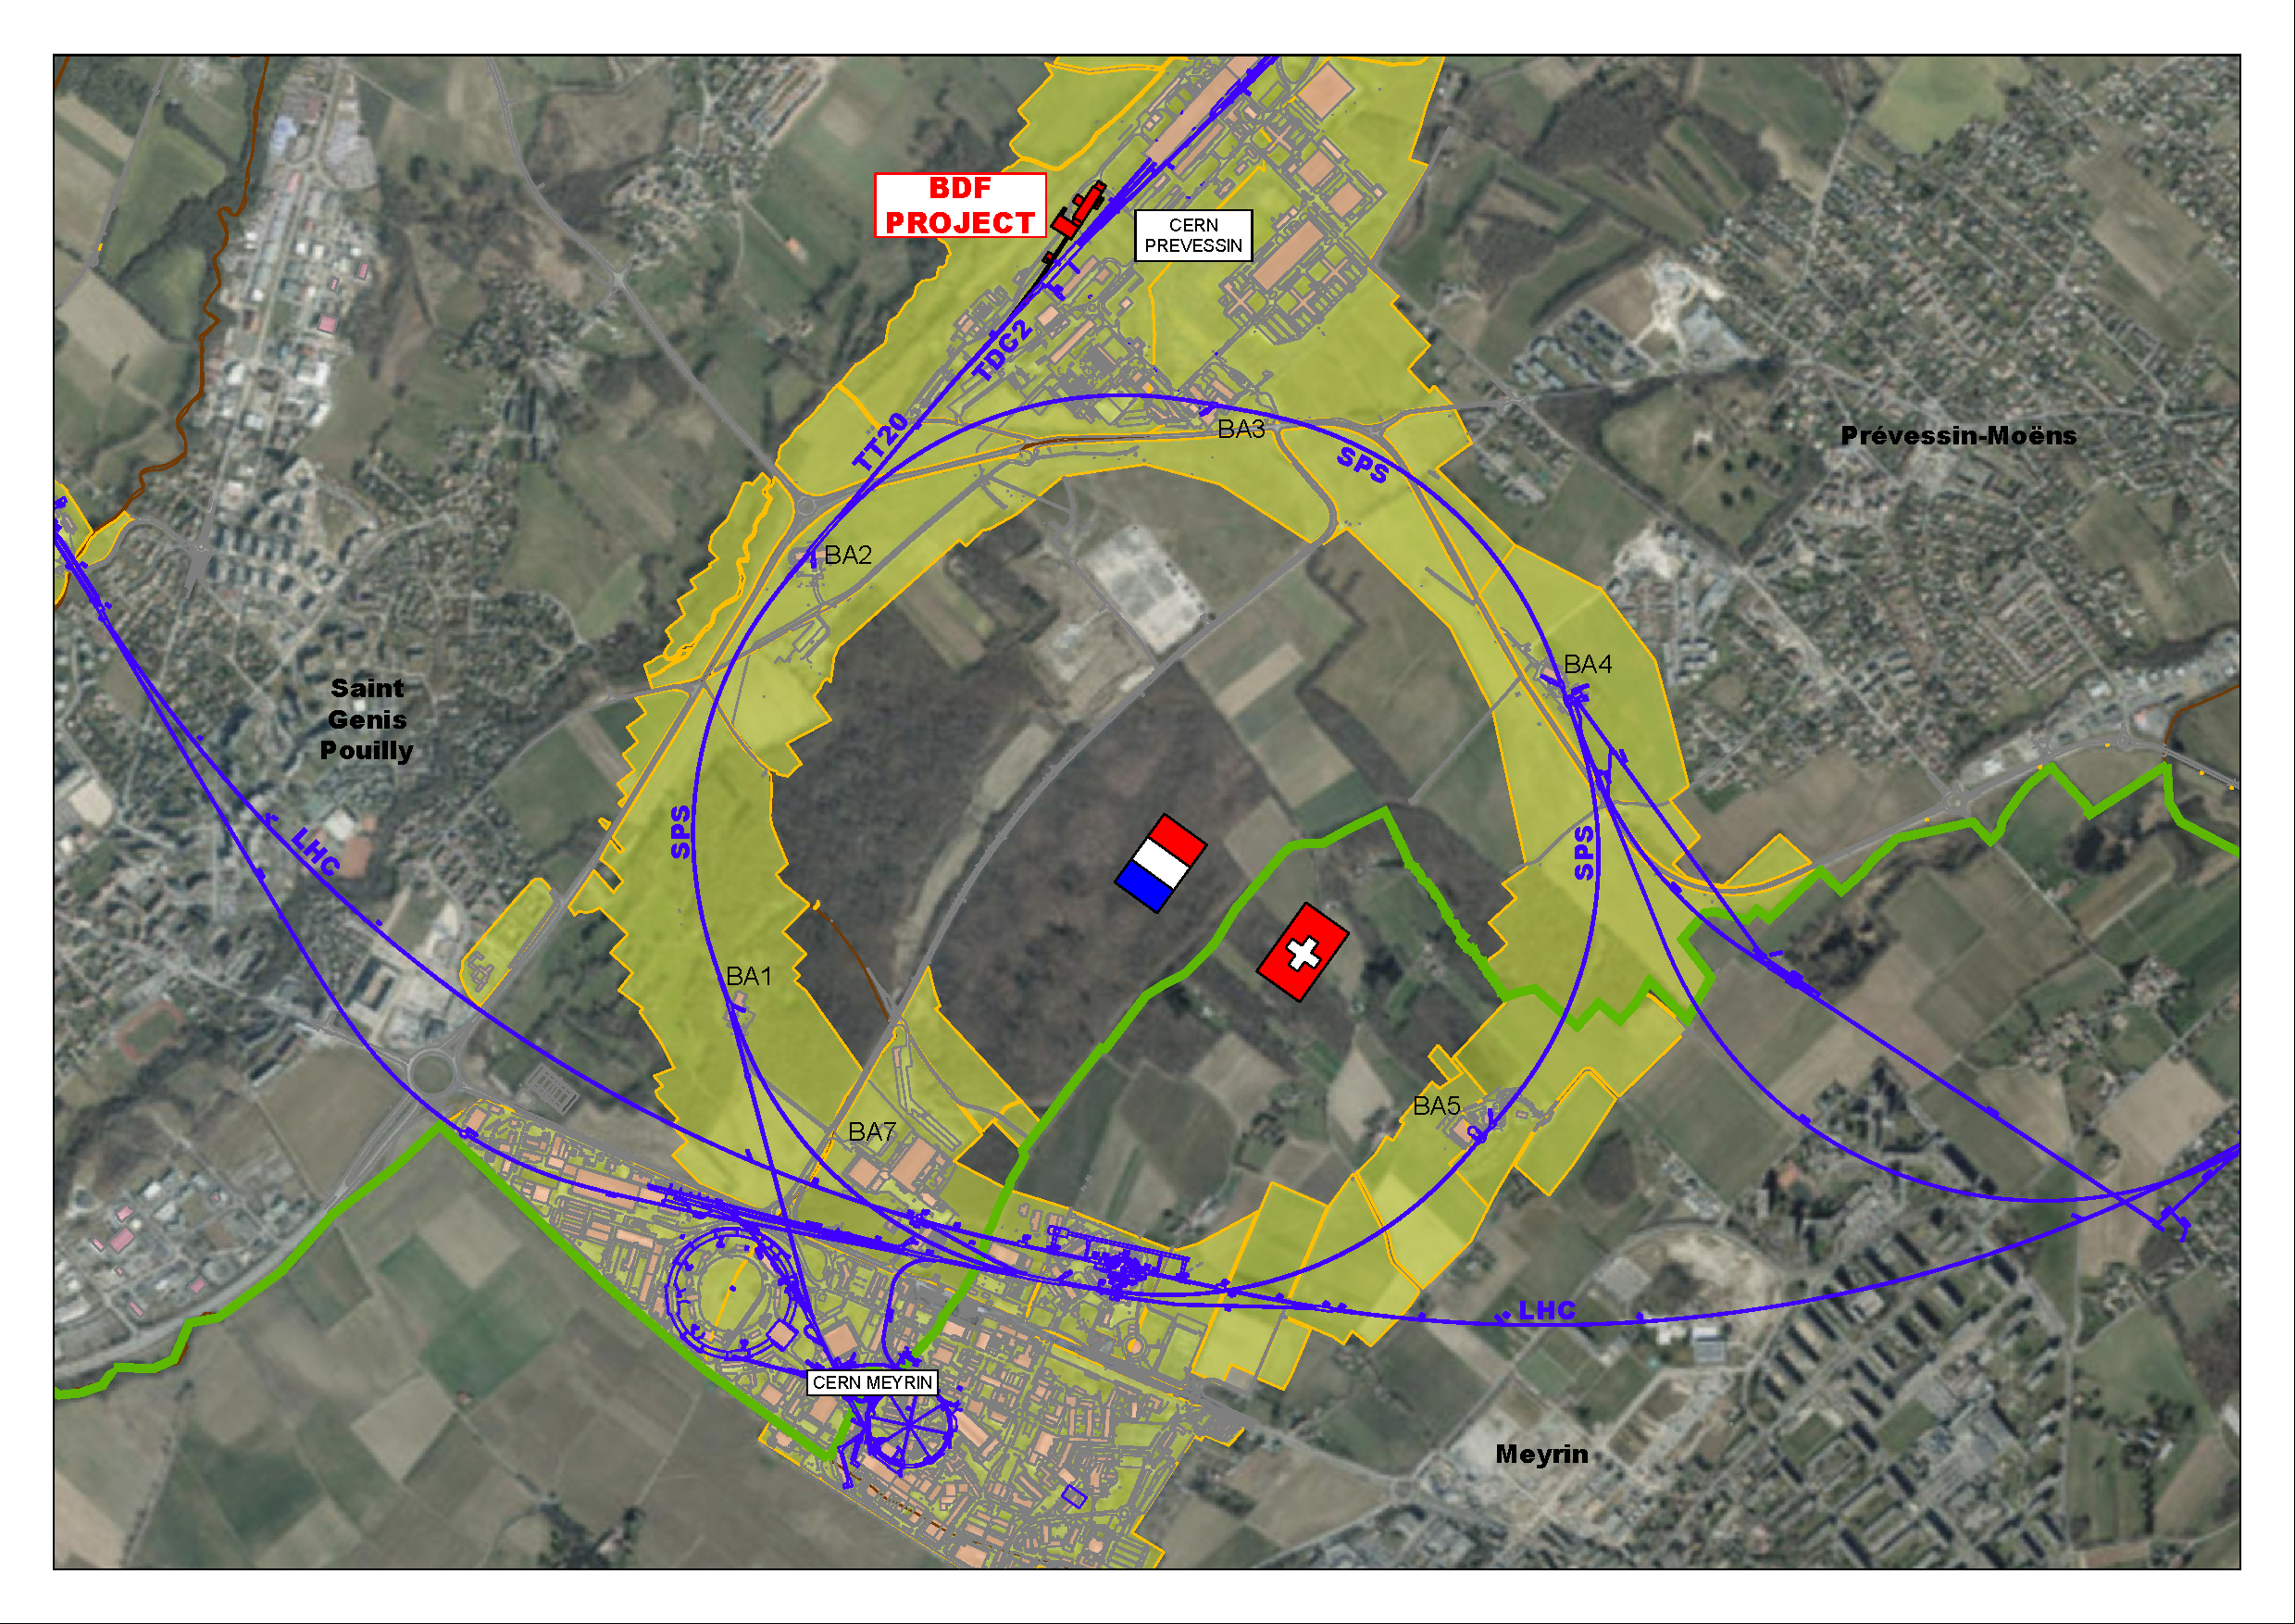
\includegraphics[width=1.0\columnwidth]{figs/BeamLine/20180529-BDF-General_figure_for_BDF_paper.pdf}
\caption{}
\label{fig:FacilityLocation}
\end{figure}

\begin{figure}[th]
\centering
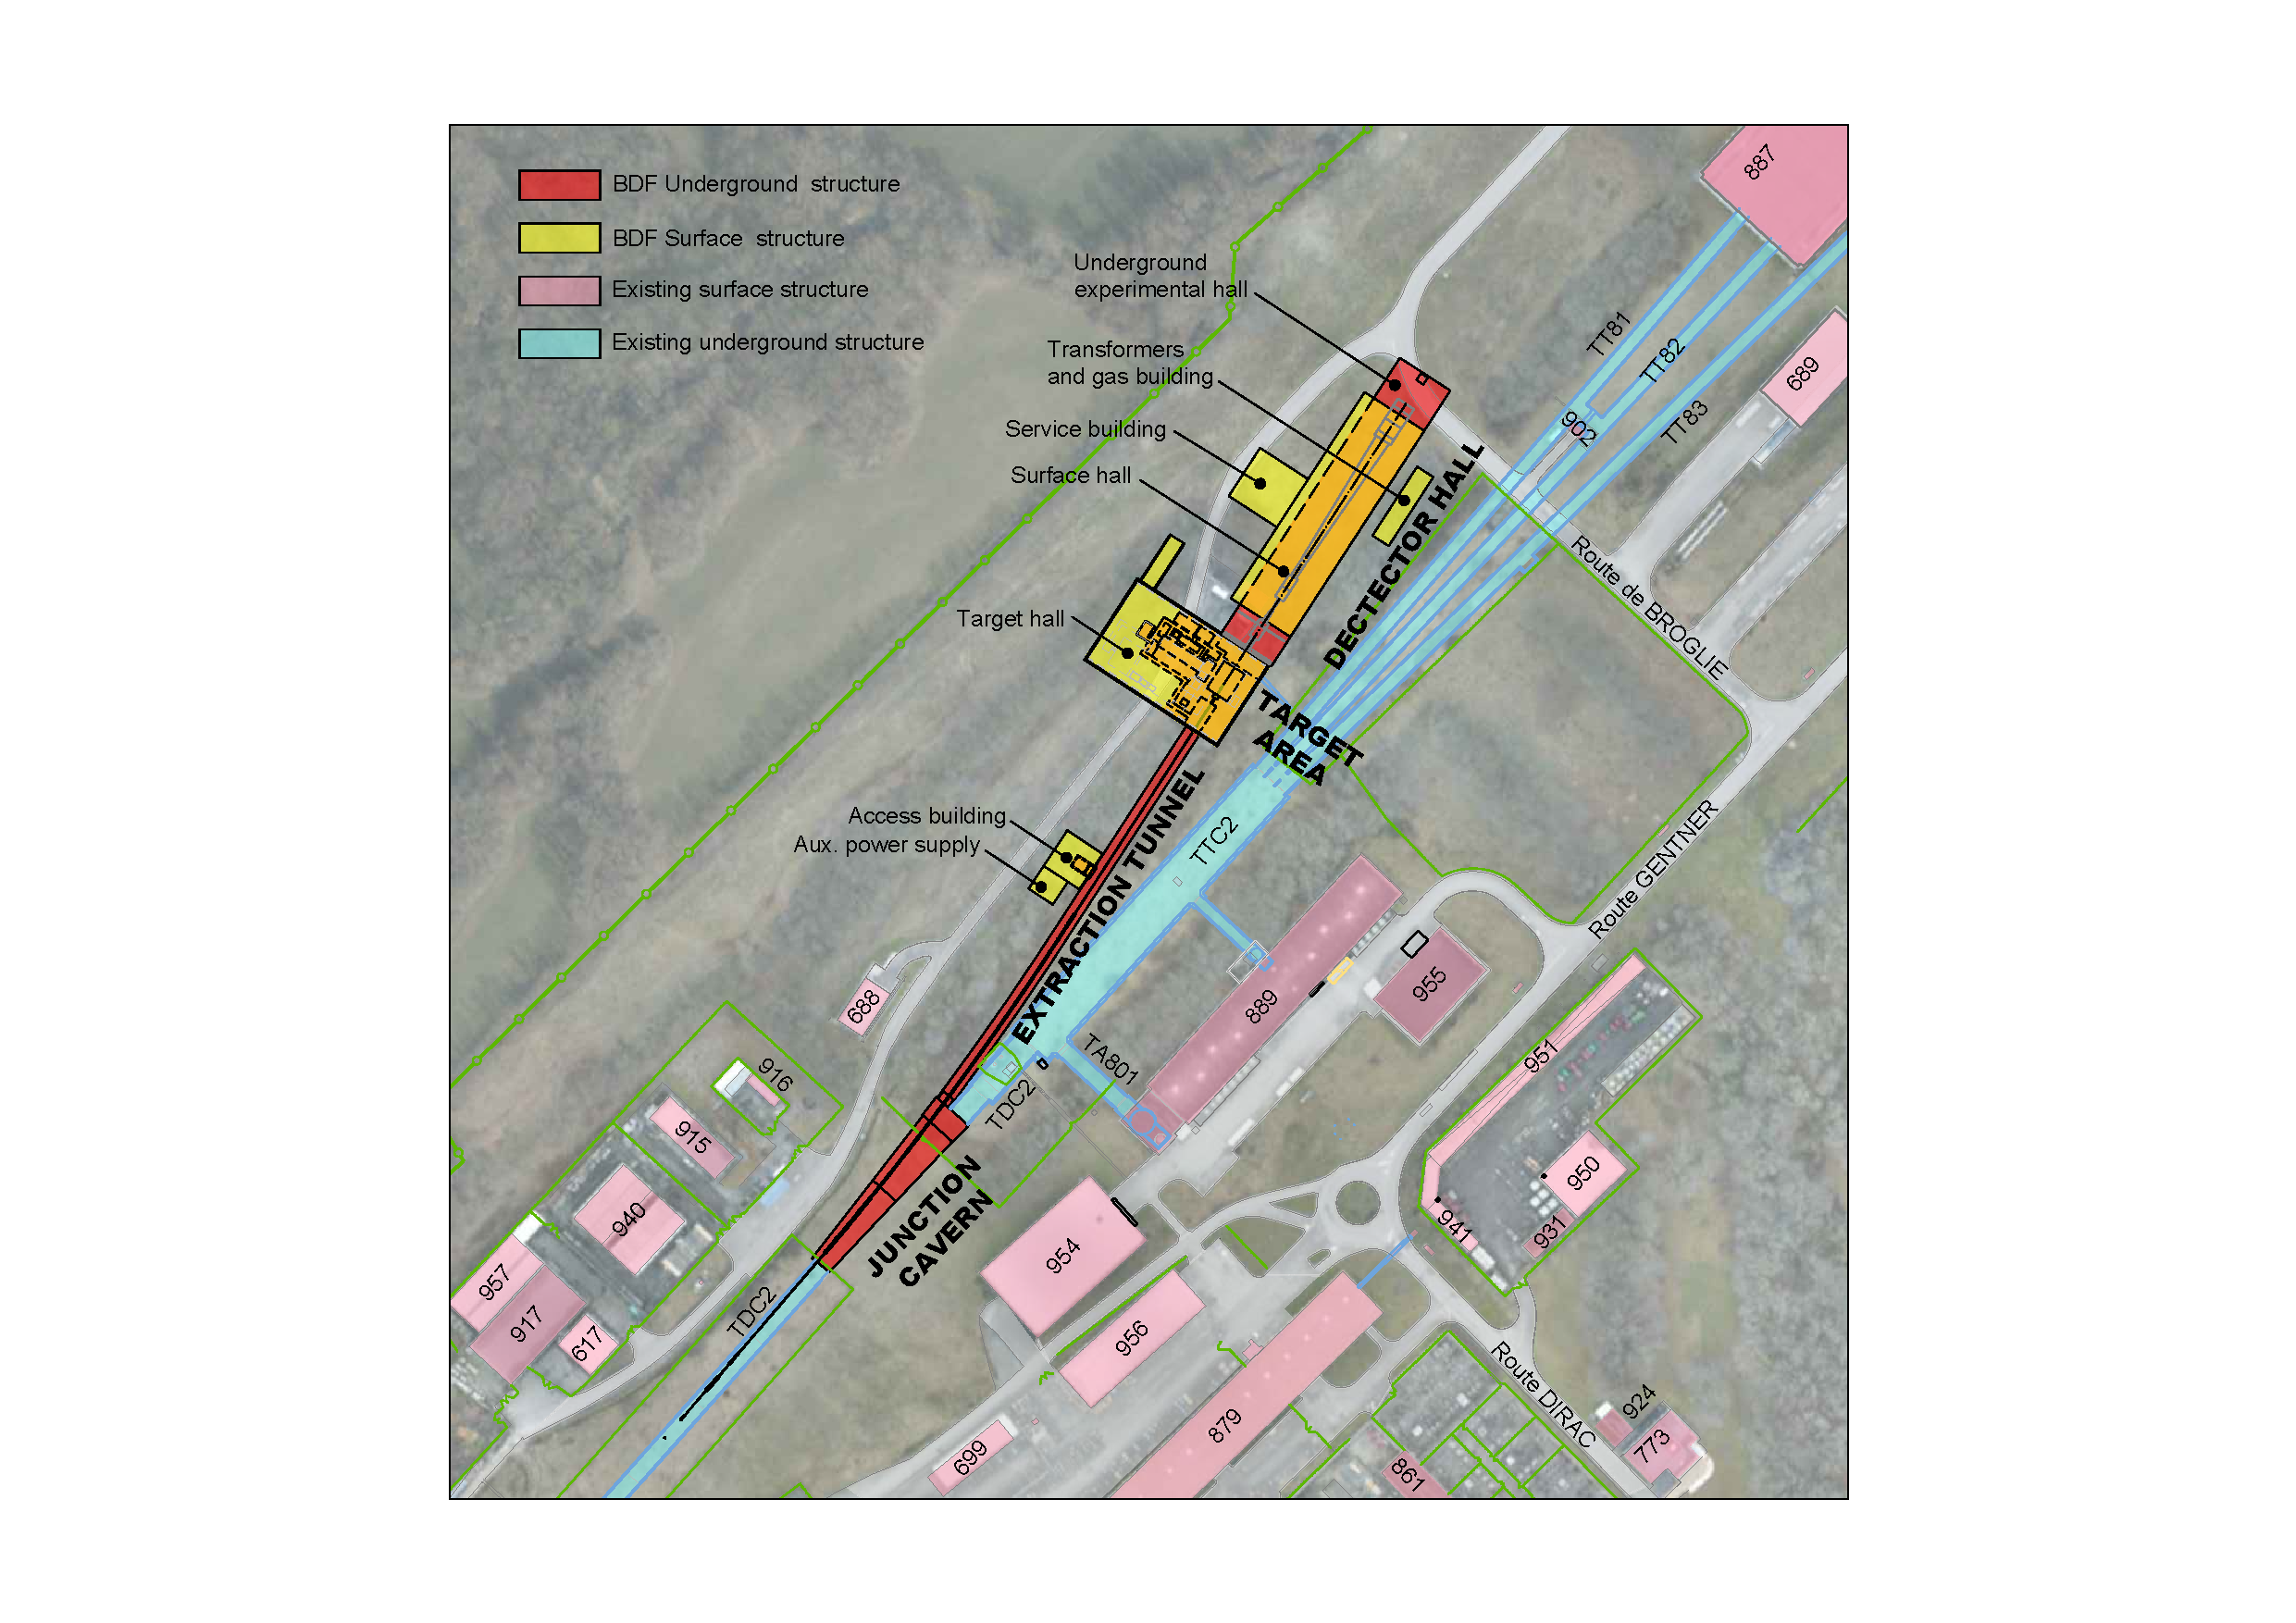
\includegraphics[width=1.0\columnwidth]{figs/BeamLine/20180529-BDF-Figure_for_BDF_paper.pdf}
\caption{}
\label{fig:FacilityLocation}
\end{figure}

\begin{figure}[th]
\centering
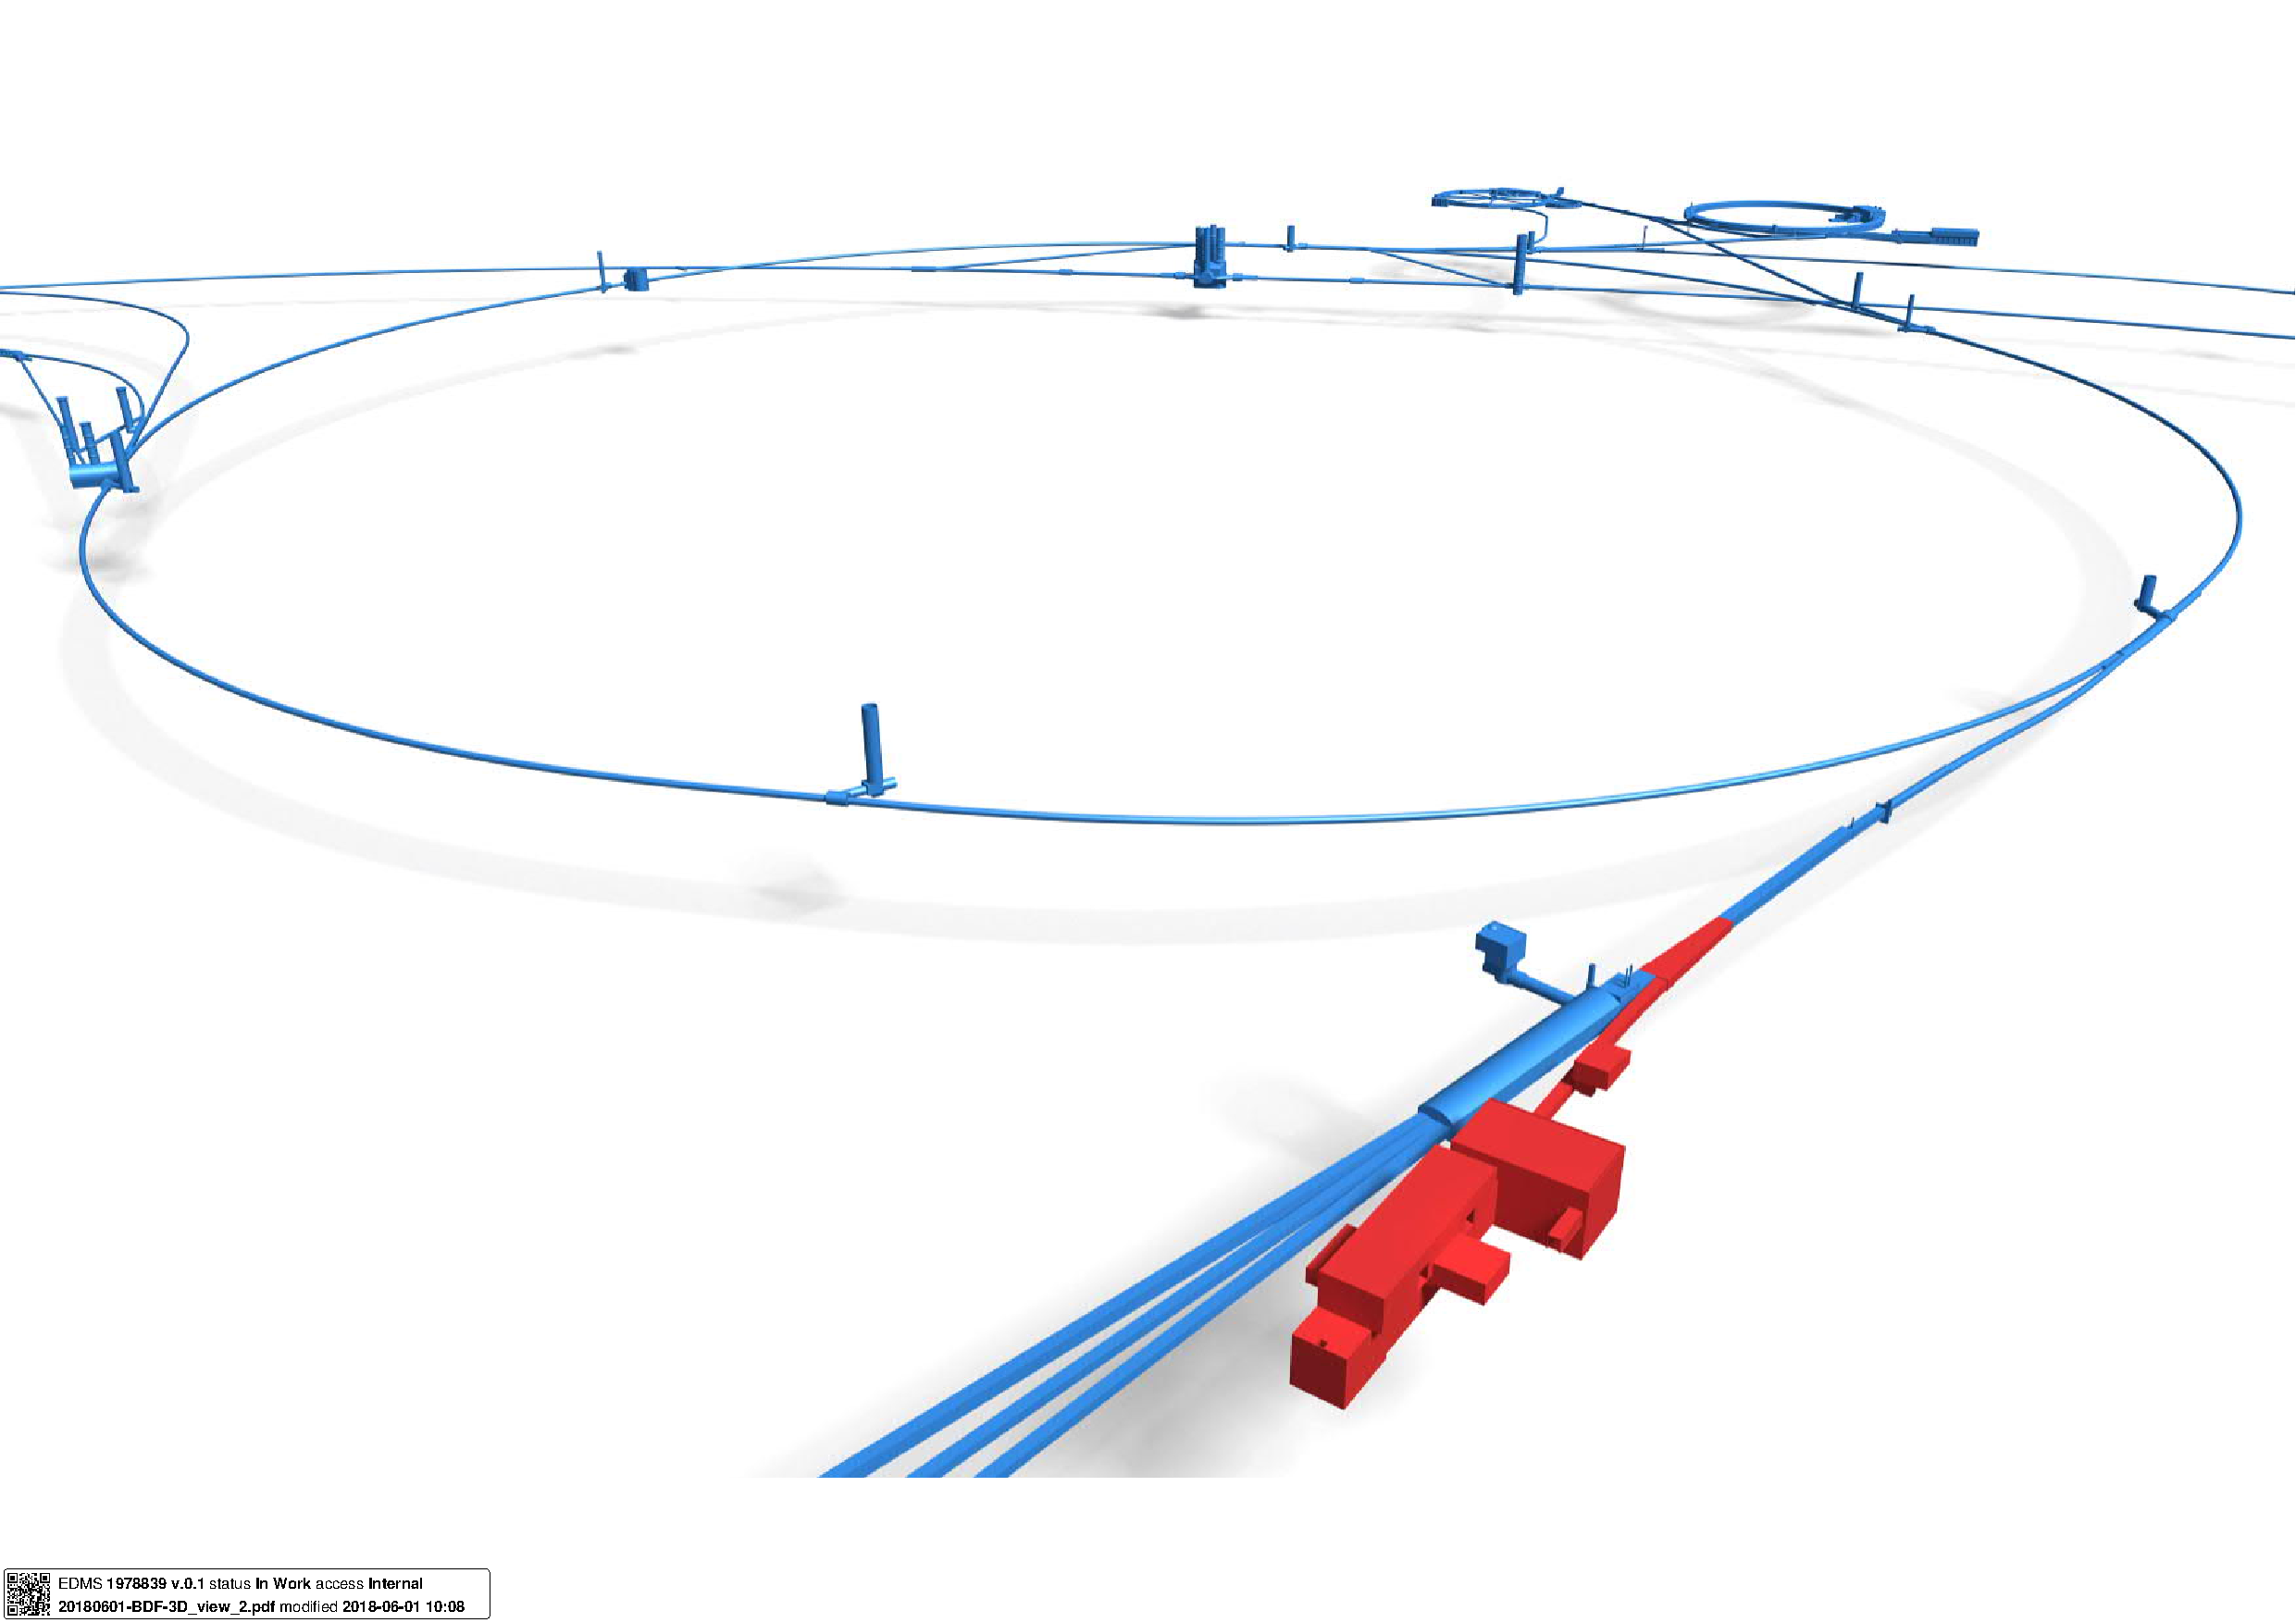
\includegraphics[width=1.0\columnwidth]{figs/BeamLine/20180601-BDF-3D_view_2.pdf}
\caption{}
\label{fig:FacilityAccComplex}
\end{figure}

The Comprehensive Design Study for the experimental facility has been carried out by the 
Beam Dump Facility working group and in its dedicated subgroups in the context of the Physics Beyond Collider Study Group in 
close collaboration with the SHiP experiment.  

Based on the request put forward in the addendum to the SHiP Technical Proposal~\cite{ref:ship_tp_add}, this study phase has 
consisted in a detailed elaboration of the SHIP operational scenario, and in a preliminary design of the main components of the 
proton delivery, the target and the target complex, and the experimental area, together with a detailed evaluation of the 
radiological aspects and mitigation. Several critical items have been prototyped to demonstrate the concepts, the new type of 
three-way combined beam splitter/kicker magnet and the target and a conceptual version of its enclosure.

In addition, it has been considered of high importance to perform a preliminary study of
the integration of the whole complex, civil engineering design and execution process in order to produce a more precise cost 
estimate and time line for the project.

A full writeup of the Comprehensive Design Study for the Beam Dump Facility is available~(\cite{ref:bdf_yellowreport} and references therein).

Assumptions and baseline parameters confirmed.

The sections below summarizes the changes, updated requirements, status and key conclusions related to the experimental facility and beam line.

Reference to feasibility studies in TP addendum and BDF working group, focus on re-optimization and updates, synthesis of conclusions BDF work



\section{Proton yield and beam delivery}

The SHiP operational scenario is based on a similar fraction of beam time as the past CERN Neutrinos to Gran Sasso (CNGS) program. The most favourable experimental conditions for SHiP are obtained with a proton beam energy of around 400 GeV. A nominal beam intensity of $4\times10^{13}$ protons on target per spill is assumed for the design of the experimental facility and the detector. In the baseline scenario, the beam sharing delivers an annual yield of $4\times 10^{19}$ protons to the SHiP experimental facility and a total of $10^{19}$ to the other physics programs at the CERN North Area, while respecting the beam delivery required by the LHC and HL-LHC . The physics sensitivities are based on acquiring a total of $2\times 10^{20}$ protons on target, which may thus be achieved in five years of nominal operation.

Significant progress has been made in the studies of techniques to reduce the beam losses 
and activation during the slow extraction process which is necessary to achieve the baseline 
intensity of $4\times 10^{19}$ protons on target per year. The current status confirms the 
intensity reach to within a factor of two, and further techniques presently under deployment 
are  aiming to provide the additional reduction to allow the full intensity.

\subsection{Operation with slow-extraction in bunched mode}

SHiP profits from the unique feature in the SPS of slow extraction of a de-bunched beam over a timescale of around a second. It allows tight control of combinatorial background, and allows diluting the large beam power deposited on the proton target both spatially and temporally. Should an observation require consolidation, a second mode of operation with slow extraction of bunched beam is also foreseen in order to further increase the discrimination between the signature of a Light Dark Matter object, by measuring their different times of flight,  
%in the mass range $0.5{-}6~\gevcc$ 
and background induced by neutrino interactions.

\section{Target system}

Target extended from 10 to 12 interaction lengths, radius changed from square block 30x30 to cylindrical with radius of 12.5cm.

% SHiP uses a target of 12 interaction lengths of molybdenum-tungsten 
% which has been designed to cope with % the large beam power and which 
% maximize the production % of charm and beauty hadrons, and the 
% production and % interactions of photons, while minimizing the production 
% of neutrinos from pion and kaon decays. The infrastructure complex to 
% house the proton target with the associated services and remote handling, 
% and which is fully compatible with the radiation protection and 
% environmental considerations, has been taken through an advanced feasibility 
% study.

\section{Updated experiment layout}

The main experimental challenge concerns the requirement of highly efficient reduction of beam-induced backgrounds to below $0.1$ events in the projected sample of $2\times 10^{20}$ protons on target. To this end, the experimental configuration includes a unique design of a muon shield based on magnetic deflection to reduce the flux of muons emerging from the target by six orders of magnitude in the detector acceptance. 

The SHiP experiment incorporates two complementary apparatuses. The first detector
immediately downstream of the muon shield consists of an emulsion based spectrometer optimised for recoil signatures of hidden sector particles and $\tau$ neutrino physics.


\subsection{Magnetization of the target hadron stopper}
Contract and activity with RAL

\subsection{Free-standing Muon shield}

The design and performance of the muon shield poses certain technological challenges. These 
include how to best assemble sheets of Grain Oriented steel without disrupting the magnetic 
circuit, how to cut the GO sheets into desired configurations, and how to best connect the 
GO sheets to achieve the desired stacking factor. In order to address these questions a 
prototyping campaign is underway.

The design of the muon shield and the residual rate of muons depends on the momentum 
distribution of the muons produced in the initial proton collision. The latest shield 
optimisation and rate estimates were performed using \texttt{PYTHIA} simulations. In order 
to validate these simulations a test beam campaign is starting in July to measure the muon 
flux using a replica of SHiP's target. Further details can be found in Ref.~[SHiP-EOI-016]. 
Depending on the outcome of this test beam campaign, a further optimisation of the 
shield configuration will be performed.

\begin{figure}[thbp]
\centering
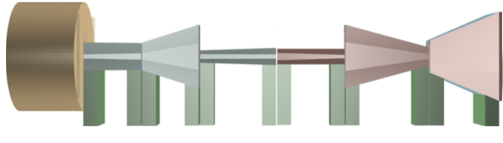
\includegraphics[width=1.0\columnwidth]{figs/BeamLine/shield_YZview.png}
\caption{Side view of the optimized muon shield magnets.}
\label{fig:shieldSideView}
\end{figure}

\begin{figure}[thbp]
\centering
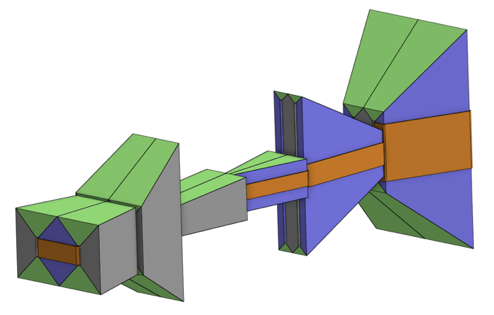
\includegraphics[width=0.8\columnwidth]{figs/BeamLine/shield_3dview.png}
\caption{3D view of the optimized muon magnetic shield.}
\label{fig:shieldSideView}
\end{figure}

\begin{figure}[thbp]
\centering
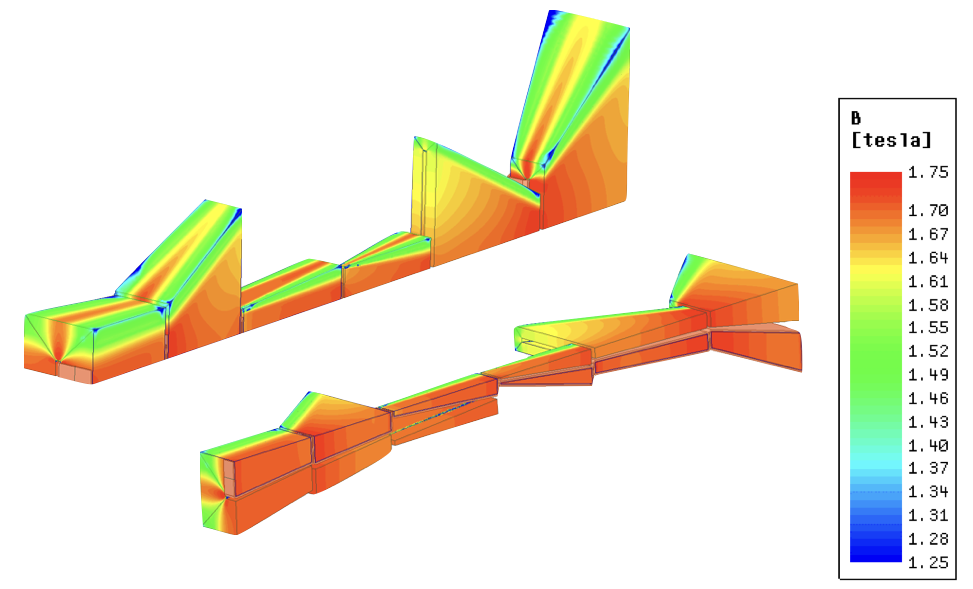
\includegraphics[width=0.8\columnwidth]{figs/BeamLine/shield_field_quadrant.png}
\caption{Modelled magnetic field distribution with nominal field intensity set to 1.7T. Quadrant cut out is shown.}
\label{fig:shieldMagneticField}
\end{figure}

\begin{figure}[thbp]
\centering
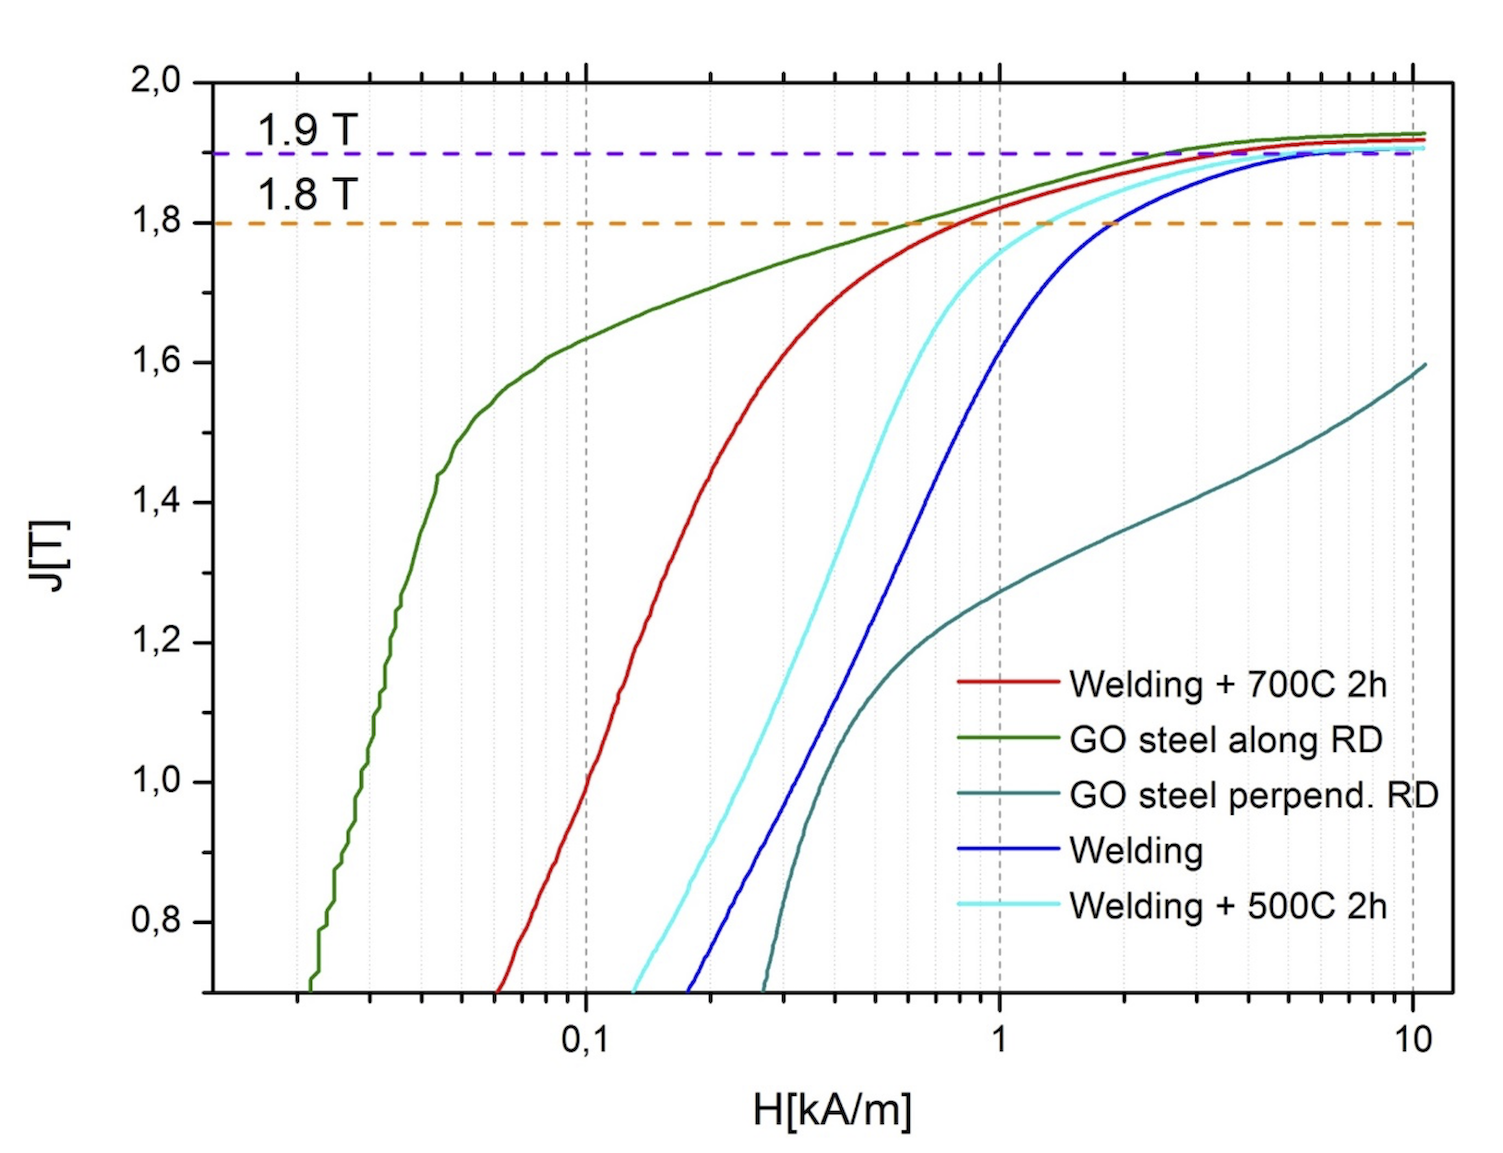
\includegraphics[width=0.8\columnwidth]{figs/BeamLine/go_steel_annealing.png}
\caption{Measured magnetic properties of the Grain Oriented steel batch: unprocessed sample along (green) and perpendicular (dark green) to rolling direction,
after the welding (blue), after the following annealing at $500^\circ$C (cyan) and $700^\circ$C (red).}
\label{fig:goSteelAnnealing}
\end{figure}

\begin{figure}[thbp]
\centering
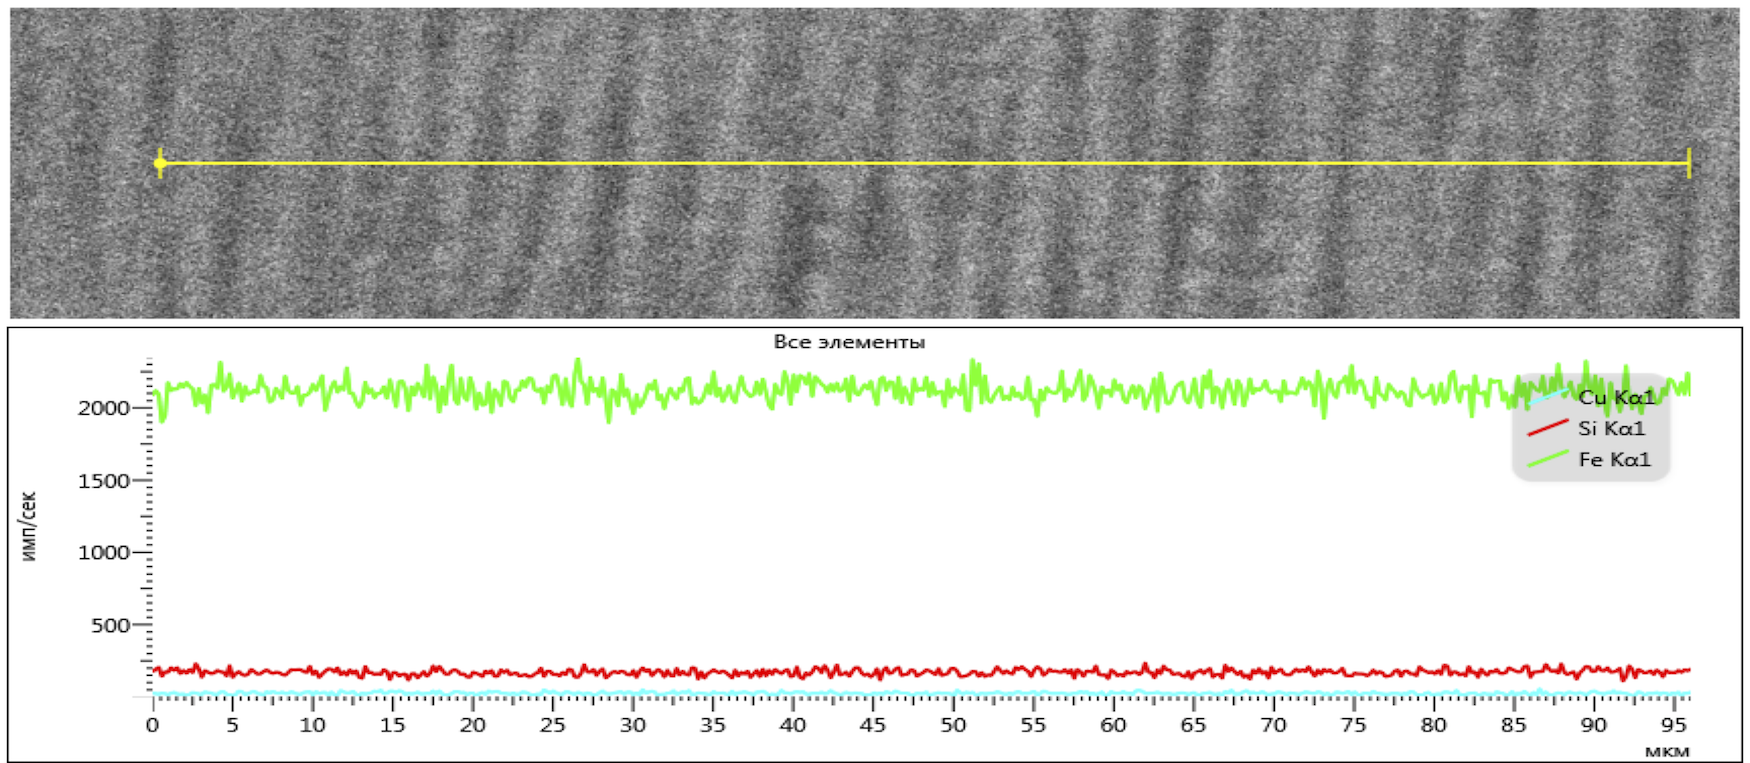
\includegraphics[width=0.45\columnwidth]{figs/BeamLine/carbon_structure.png}
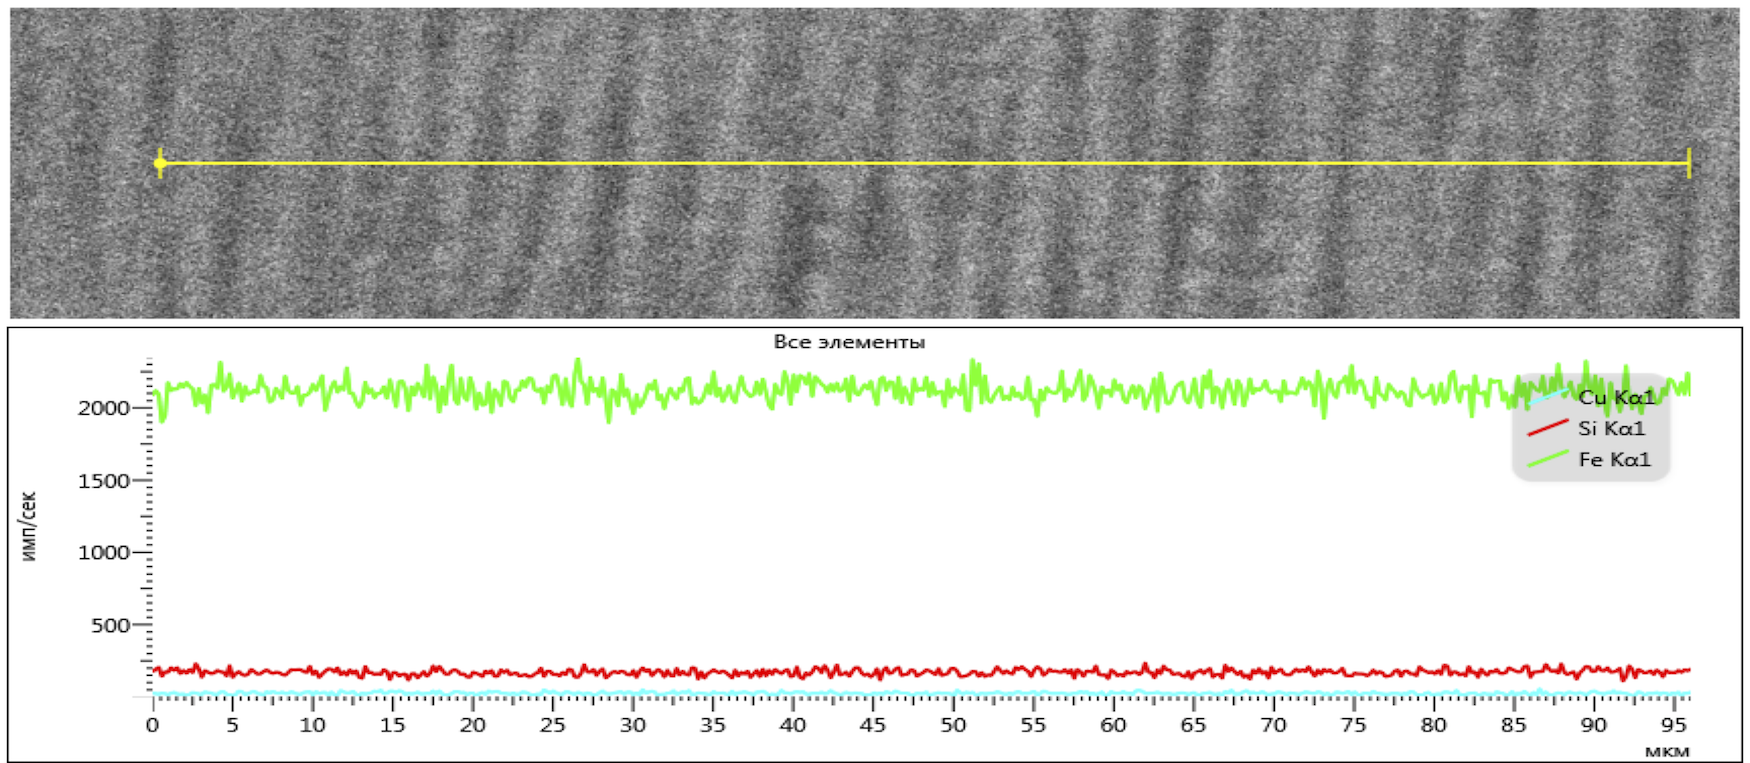
\includegraphics[width=0.45\columnwidth]{figs/BeamLine/carbon_structure.png}
\caption{Carbon structure in the welded joint before (left) and after (right) \em{(to be updated)} annealing.}
\label{fig:goCarbonStructure}
\end{figure}

\begin{figure}[thbp]
\centering
%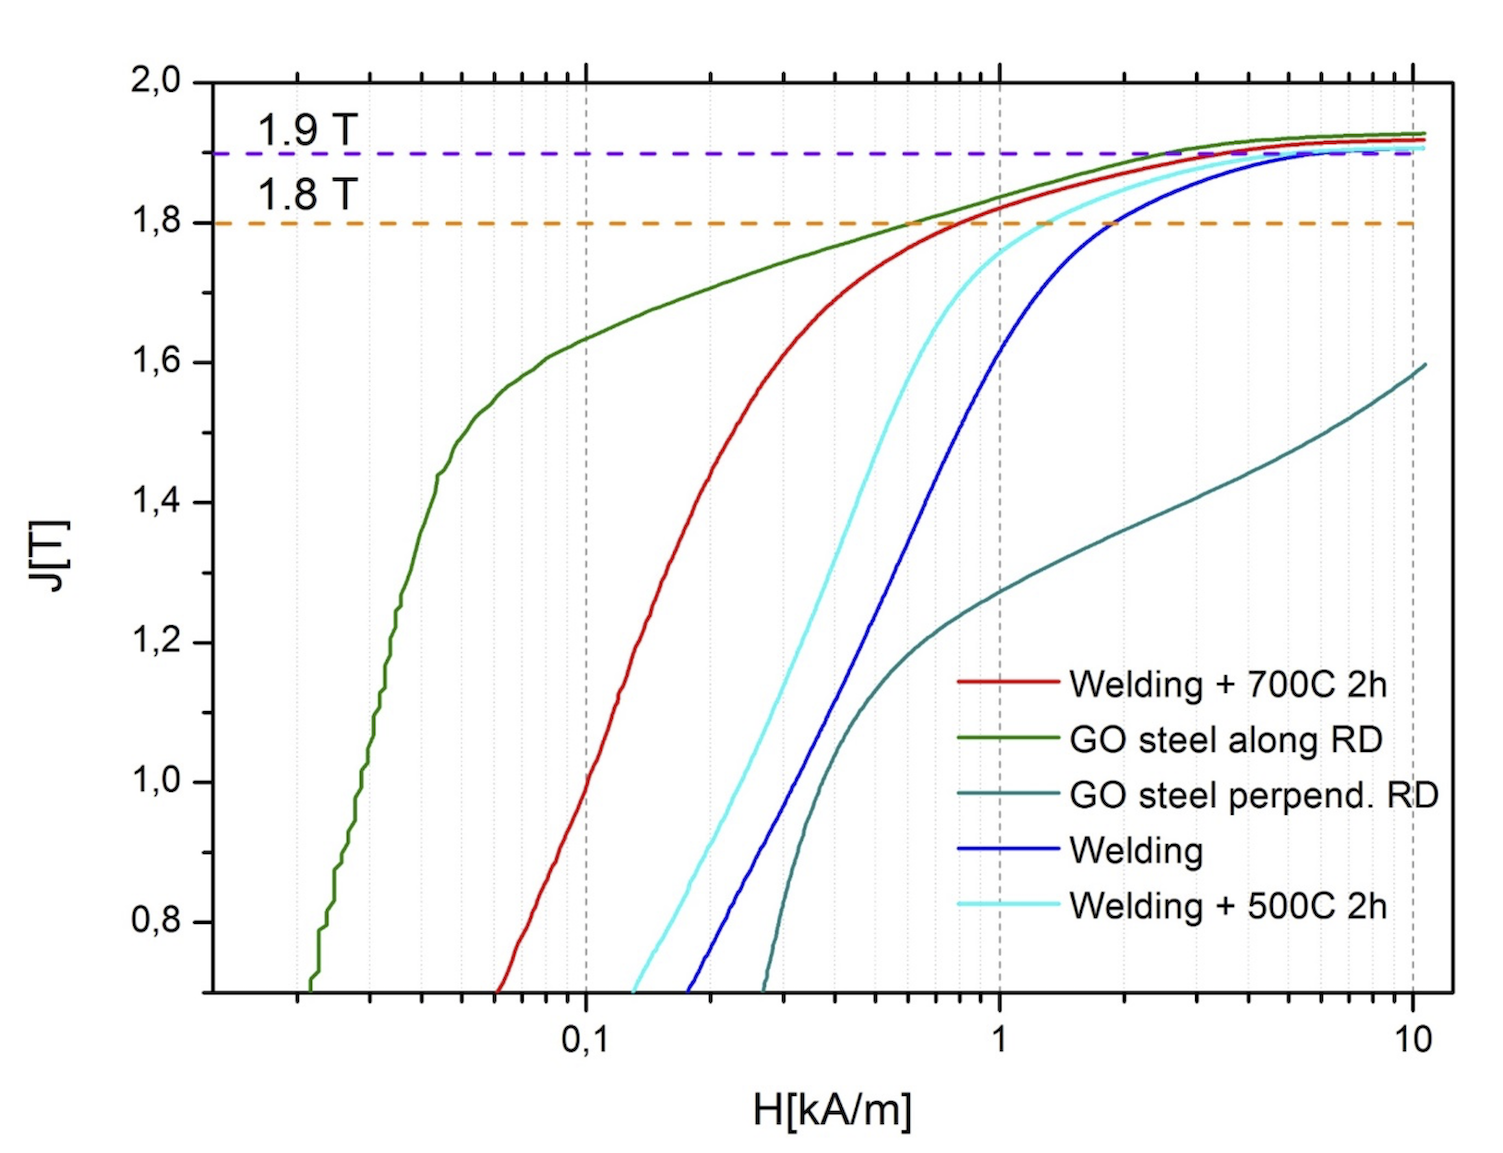
\includegraphics[width=1.0\columnwidth]{figs/BeamLine/go_steel_annealing.png}
\caption{Simulated hit rates caused by muons passing magnetic shield. Comparison of  ideal magnetic field setup (red) and realistic magnetic field (blue).}
\label{fig:shieldHitsMap}
\end{figure}

\begin{figure}[thbp] 
\centering
%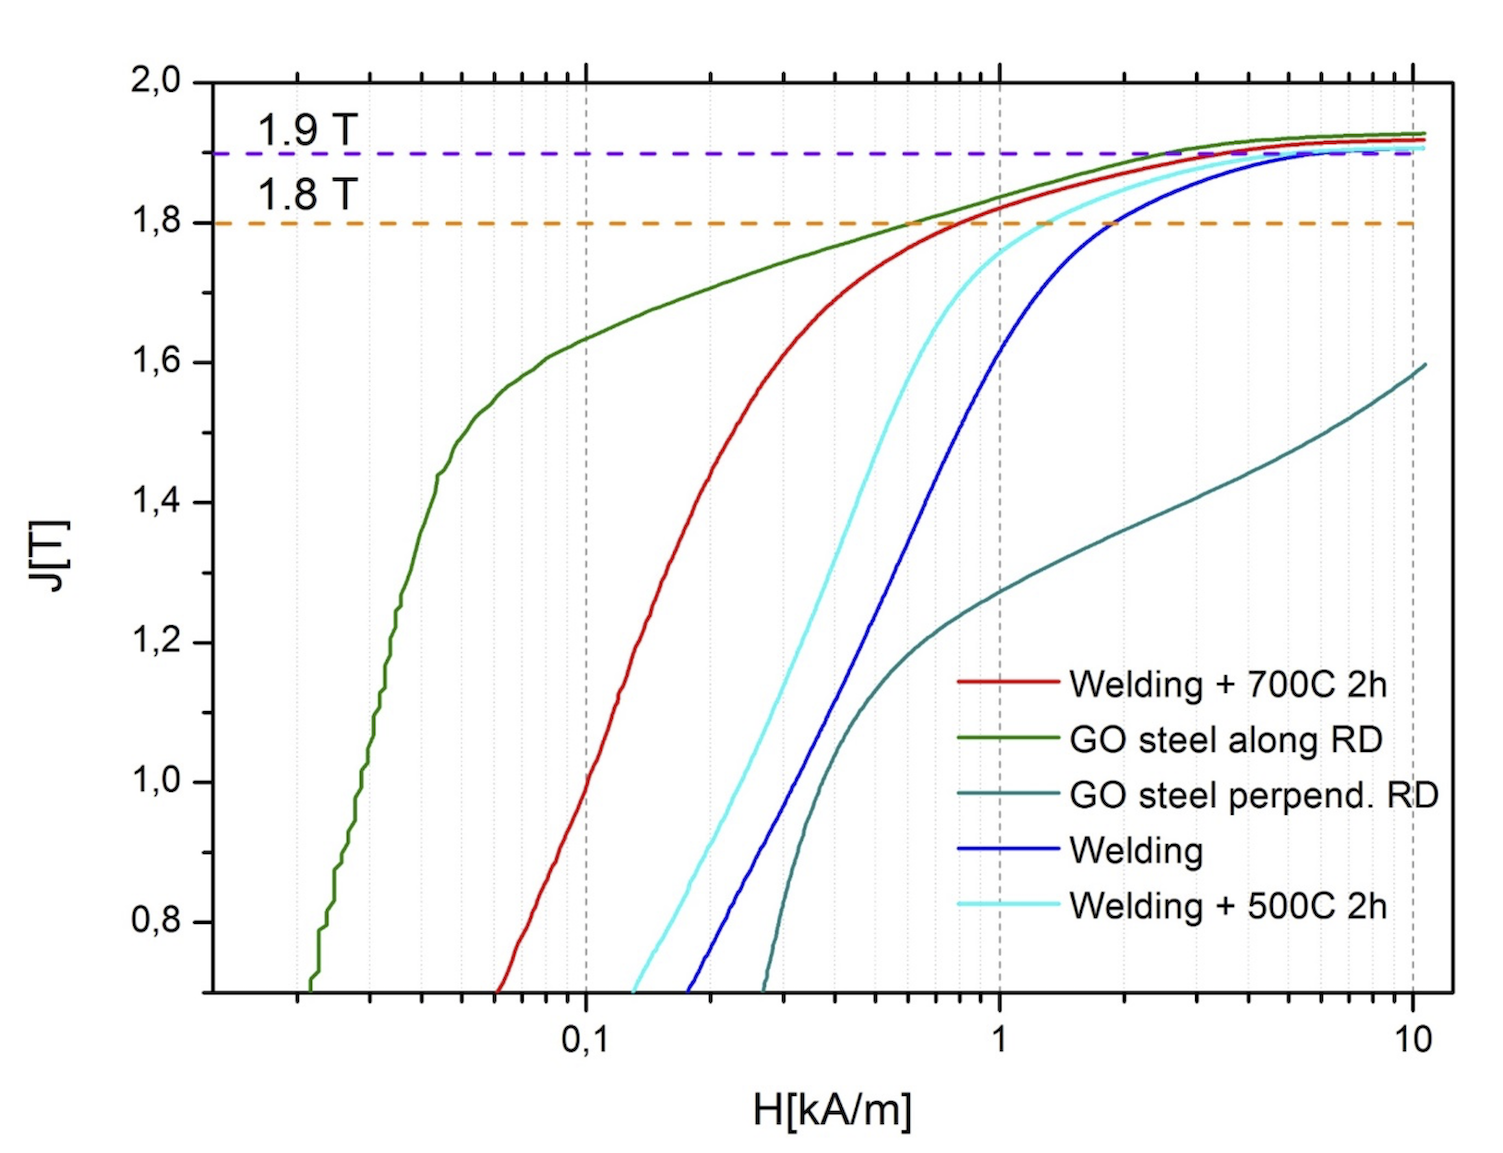
\includegraphics[width=1.0\columnwidth]{figs/BeamLine/go_steel_annealing.png}
\caption{Reconstructed track rates caused by muons passing magnetic shield. Comparison of  ideal magnetic field setup (red) and realistic magnetic field (blue).}
\label{fig:shieldTracks}
\end{figure}



\subsection{Vacuum vessel}
Baseline is a ....
Consist of several sections


The preliminary studies of the vacuum system for the approximately 1750 $m^3$ SHiP vacuum vessel 
shows that the requirements can be satisfied with a system of combined root-screw pumps, piezo 
and membranes gauges for pressure monitoring and manual valves for operation and venting 
purposes~\cite{ref:vacuumsystem}(EDMS 2000025). 
A low outgassing epoxy paint is considered to be deposited on the steel surface under vacuum in 
order to reduce the surface outgassing. The longitudinal vacuum forces which are taken into 
account in the design of the vacuum chamber are around 300t. 



\section{Experimental Area and Infrastructure}

\begin{figure}[th]
\centering
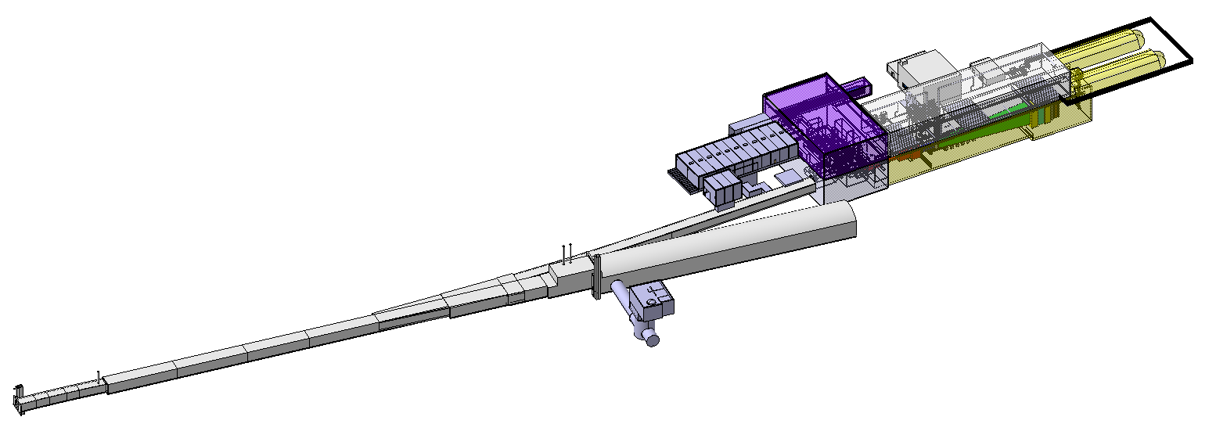
\includegraphics[width=0.9\columnwidth]{figs/BeamLine/2018_09_FacilityOverview.png}
\caption{}
\label{fig:FacilityOverview}
\end{figure}

\begin{figure}[th]
\centering
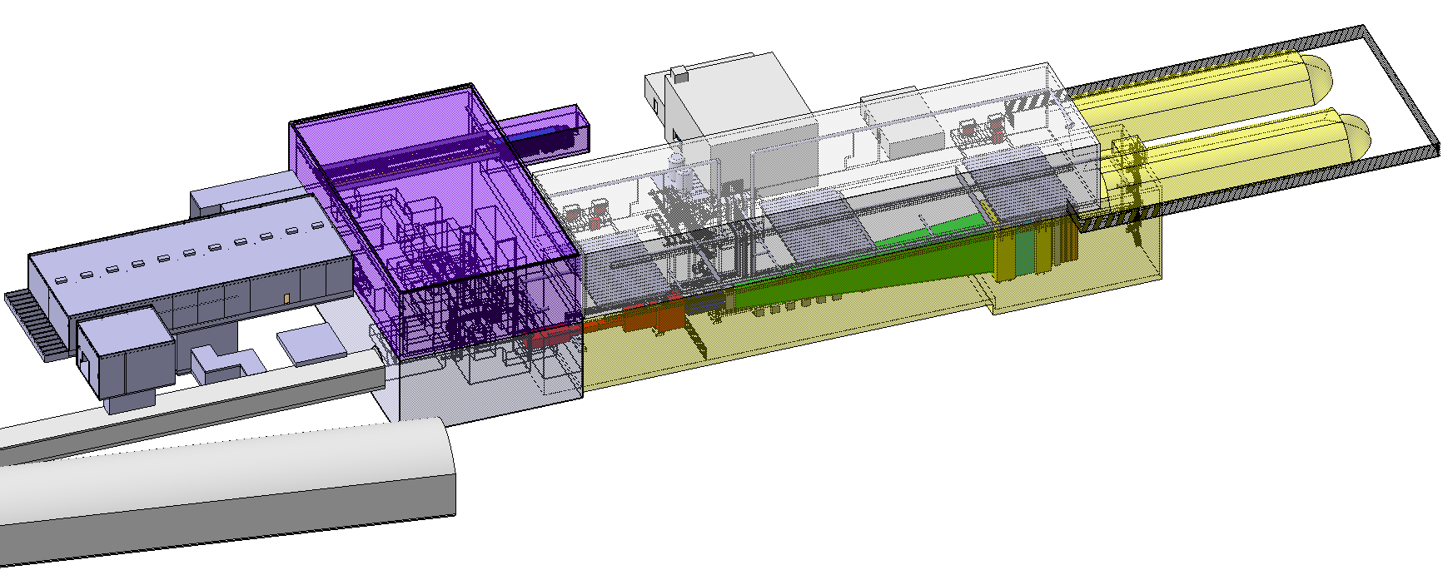
\includegraphics[width=0.9\columnwidth]{figs/BeamLine/2018_09_ExperimentalAreaOverview.png}
\caption{}
\label{fig:ExperimentalAreaOverview}
\end{figure}





\section{Potential siting of a search for Lepton Flavour Violation experiment}

(Pictures from presentation at BDF WG)

Motivation (yield)

From the beam optics point of view, several locations can provide the required beam conditions 
and the beam drift space to accommodate the detector along the new $200~m$ transfer line between 
the TDC2 switch yard cavern and the BDF target station without affecting the location of the BDF 
experimental area and without significant changes to the configuration of the beam line. The 
choice is instead driven by considerations related to the civil engineering in the vicinity of 
the existing installations, radiological protection, and to access and transport requirements 
above ground and underground.  Lateral space is required on both sides for shielding in order 
to limit the radiation exposure of the surrounding underground area to levels typical for the 
rest of the beam line.

The preferred location under study is situated $60~m$ upstream of the BDF target bunker. An 
access and service complex for the transfer line is already foreseen at this location. It would 
be extended and reconfigured to include a bypass tunnel, the detector bunker, service cavern 
and the required surface complex. 

By a modest reconfiguration of the existing beam elements, the location provides a beam spot of 
$\sigma_x=4.4~mm ~\times \sigma_y=1.1~mm$ and a drift space of $20~m$ to implement the detector 
and the shielding. A compensator magnet is foreseen to allow the experimental dipole magnet and 
the need to swap polarity. The downstream dilution system which is required to sweep the beam 
in a circle on the BDF target to dilute the beam power will have to be twice as strong in this 
configuration.

A first check of the characteristics of the proposed target configuration and beam induced 
effects on the material has revealed no showstopper. The target and the silicon-pixel detector 
will share a common closed volume containing an inert gas in circulation to prevent radiation 
induced corrosion and to ensure external cooling of the target and the detector.

A preliminary FLUKA study of the radiological aspects has been performed. It confirms that the 
radiation environment will be very challenging for the detectors. Remote handling will be 
required to move the detectors out of their data taking position into an adjacent service cavern 
for interventions. A shielding wall will separate the service cavern from the detector bunker 
during operation. No access is allowed underground during operation. An important challenge 
concerns preventing irradiation of the downstream beam elements due to radiation leakage through 
the whole in the shielding for the beam line.

A preliminary check of the surrounding environment shows no problems with respect to 
environmental limits or fluxes in neighbouring underground areas at the North Area, but this 
requires further studies. The additional flux of muons and neutrinos which enter the SHiP 
experiment will be studied as soon as the TauFV experimental configuration reaches more maturity.




%%%%%%%%%%%%%%%%%%%%%%%%%%%%%%%%%%%%%%%%%

%Since CERN currently has no experimental facility which is compatible with the full potential of the SPS, SHiP requires a new facility. CERN's North Area has a large space next to the SPS beam transfer lines which is largely free of structures and 
%underground galleries, and is entirely located on the current CERN territory. The proposed implementation is based on minimal modification to the SPS complex and maximum use of the existing beam lines. The design foresees space for future extensions.


% SHiP uses a target of 12 interaction lengths of molybdenum-tungsten 
% which has been designed to cope with % the large beam power and which 
% maximize the production % of charm and beauty hadrons, and the 
% production and % interactions of photons, while minimizing the production 
% of neutrinos from pion and kaon decays. The infrastructure complex to 
% house the proton target with the associated services and remote handling, 
% and which is fully compatible with the radiation protection and 
% environmental considerations, has been taken through an advanced feasibility 
% study.
%% KP detail i think...
%%A new type of beam splitter magnet allows switching the beam to a short new transfer line to the SHiP 
% experimental facility at the top of the TT20 transfer line, while maintaining operational all the current experimental facilities at the CERN North Area.






%The SHiP experiment incorporates two complementary apparatuses. The detector system immediately downstream of the muon shield is optimized for both recoil signatures of hidden sector particle scattering and for neutrino physics. It is based on an emulsion system interleaved with an electronic tracking system and high-density $\nu$-target layers in a magnetic field. The detector $\nu$-target mass totals ${\cal{O}}(10)~tonnes$. The emulsion spectrometer is followed by a muon identification system. This also acts as a tagger for interactions in the muon filters which may produce long-lived neutral mesons entering the downstream decay volume and whose decay may mimic signal events.
%The second detector system aims at measuring the decays of Hidden Sector particles to fully reconstructible final states as well as partially reconstructible final states that involve neutrinos. The spectrometer is designed to accurately reconstruct the decay vertex, the mass, and the impact parameter of the hidden particle trajectory at the proton target. A set of calorimeters and muon stations provide particle identification. %The system is optimized to as many final states as possible in order to be sensitive to, and discriminate between, a very wide range of models. 
%A dedicated timing detector with $\leq100~\ps$ resolution provides a measure of coincidence in order to reject combinatorial backgrounds. The decay volume is surrounded by background taggers to tag neutrino and muon interactions in the vacuum vessel walls and in the surrounding infrastructure.  %which may produce long-lived neutral SM particles, such as $K_L$ etc.

%The detector consists of a 50 m long decay volume followed by a large spectrometer with a rectangular acceptance of 5 m in width and 10 m in height. In order to suppress the background from neutrinos interacting in the fiducial volume, it is maintained at a pressure of ${\cal{O}}(10^{-3})~bar$. The spectrometer is designed to accurately reconstruct the decay vertex, the mass, and the impact parameter of the hidden particle trajectory at the proton target. A set of calorimeters and muon stations provide particle identification. The system is optimized to as many final states as possible in order to be sensitive to, and discriminate between, a very wide range of models. A dedicated timing detector with $100~ps$ resolution provides a measure of coincidence in order to reject combinatorial backgrounds. The decay volume is surrounded by background taggers to tag neutrino and muon inelastic scattering in the vacuum vessel walls which may produce long-lived neutral SM particles, such as $K_L$ etc.

% The muon shield and the SHiP detectors are housed in an underground hall $120~m$ in length and $20~m$
% width, at a depth of $\sim15~m$. 
% The proposed implementation of the SHiP experimental facility is based on minimal modification to the % SPS complex and maximum use of the existing accelerator and beam lines. All civil engineering works 
% are fully located within existing CERN land on the Prevessin site.
%%%%%%%%%%%%%%%%%%%%%%%%%%%%%%%%%%%%%%%%%


